
\documentclass[a4paper,compress]{beamer}
%\usepackage{beamerthemesplit}


\usepackage[utf8]{inputenc}
\usepackage[french]{babel}

\usepackage{array}
% \usepackage{colortbl}
% 
% \usepackage{enumerate}
% \usepackage{multirow}
% \usepackage{graphicx}
% 
\usepackage{times}
%\usepackage[T1]{fontenc}


% ---- inclusion de codes

\usepackage{listings}
\lstset{showstringspaces=false,frame=trBL,frameround=tttt,tabsize=4,basicstyle=\tiny,breaklines=true,breakatwhitespace=true}
\lstdefinestyle{bash}{language=bash}
\lstdefinestyle{Perl}{language=Perl}
\lstdefinestyle{C++}{language=C++}
\lstdefinestyle{DTD}{language=XML}
\lstdefinestyle{XML}{language=XML,usekeywordsintag=false,markfirstintag=true}
\newcommand{\includecode}[2]{\lstinputlisting[style=#1]{#2}}
\lstnewenvironment{code_bash}{\lstset{style=bash}}{}
\lstnewenvironment{code_perl}{\lstset{style=Perl}}{}
\lstnewenvironment{code_cpp}{\lstset{style=C++}}{}
\lstnewenvironment{code_dtd}{\lstset{style=DTD}}{}
\lstnewenvironment{code_xml}{\lstset{style=XML}}{}

\newcommand{\textcode}[1]{{\small {\tt #1}}}


\newenvironment{clp}[1][\small]
{\begin{block}{#1 Purpose}#1}
{\end{block}}

\newenvironment{tabfn}[1][\small]
{\begin{block}{#1 Main virtual methods}#1\begin{tabular}{>{\tt}l>{//\hspace{5mm}}l}}
{\end{tabular}\end{block}}

\newenvironment{cli}[1][\small]
{\begin{block}{#1 Instances}#1\begin{itemize}}
{\end{itemize}\end{block}}

\newenvironment{cltodo}[1][\small]
{\begin{block}{#1 ToDo}#1\begin{itemize}}
{\end{itemize}\end{block}}


% \mode<presentation>
% {
%   \usetheme{Warsaw}
% }



\title{SOFA: a modular yet efficient physical simulation architecture}
\author{François Faure, INRIA}
% \institute{ LJK, Grenoble }
% \date{September, 2006}
\date{October 2012}

\AtBeginSection[]{
\begin{frame}
 \frametitle{Outline}
 \tableofcontents[currentsection]
\end{frame}
}

\begin{document}

\begin{frame}
  \maketitle
%\vspace{-28mm}
\begin{center}
 %
\includegraphics[width=\linewidth]{logos.png}
\newcommand{\logoheight}{10mm}
 
\includegraphics[height=\logoheight]{inria-logo.png} \\ \vspace{10mm}~ \\
 
\includegraphics[height=\logoheight]{alcove-logo.jpg}
 
\includegraphics[height=\logoheight]{evasion-logo.png}
 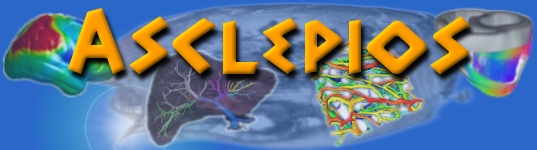
\includegraphics[height=\logoheight]{asclepios-logo.jpg}
 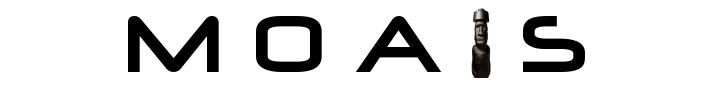
\includegraphics[height=5mm]{moais-logo.png}
\end{center}
%\tableofcontents

\end{frame}

% Etat de l'art
% Linear solutions
% Matrix factoring
% Tree
% layered models
% Extended tree
% Matrix-vector product in etended trees

\section{Motivation}

\begin{frame}
\frametitle{The complexity of physical simulations}
\begin{center}
 \includegraphics[width=0.7\linewidth]{anatomical_structures.jpg}
\end{center}
Material, internal forces, contraints, contact detection and modeling, ODE solution, visualization, interaction, etc.
\end{frame}

%----------------------------------------------------
\begin{frame}
\frametitle{Simulation platforms}
\begin{itemize}
\item Current platforms (ODE, Havok, PhysX, etc.) provide:
\begin{itemize}
\item limited number of material types
\item limited number of geometry types
\item no control on collision detection algorithms
\item no control on interaction modeling
\item few (if any) control of the numerical models and methods.
\item no control on the main loop
%\item few (if any) parallelism
\end{itemize}
\item We need much more !
\begin{itemize}
 \item models, algorithms, scheduling, visualization, etc.
\end{itemize}

\end{itemize}
\end{frame}




%%%===================================================================
\section{Modularity}
%%%===================================================================


%----------------------------------------------------
\begin{frame}
\frametitle{A generic approach}
\begin{itemize}
\item Behavior model: all internal laws
\item Others: interaction with the world
\item Mappings: relations between the models (uni- or bi-directional)
\end{itemize}
\begin{center}
 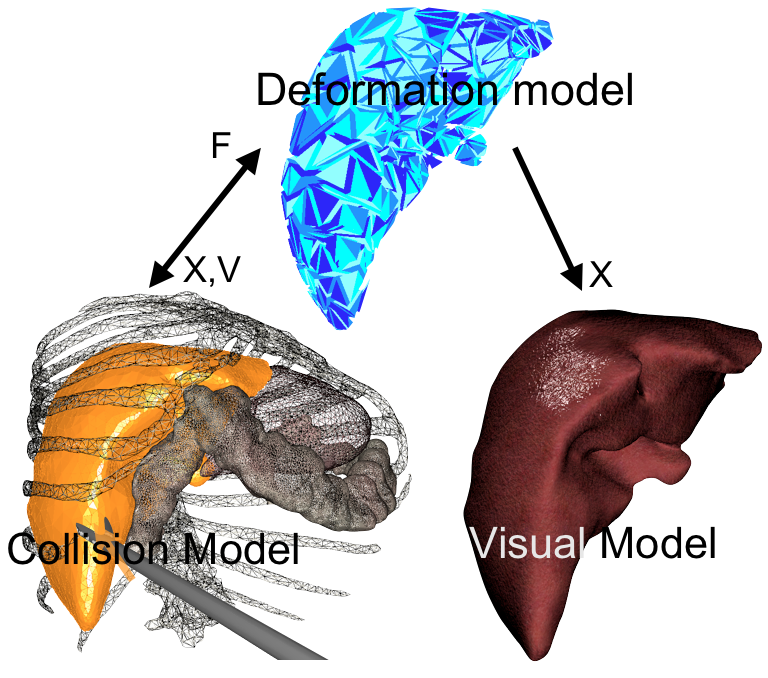
\includegraphics[width=0.5\linewidth]{NewLiverMap.png}
\end{center}

\end{frame}



%-----------------------------------------
\begin{frame}[fragile]
\frametitle{Animation of a simple body}
\begin{columns}

\column[t]{0.5\linewidth}
\begin{itemize}
\item a liver
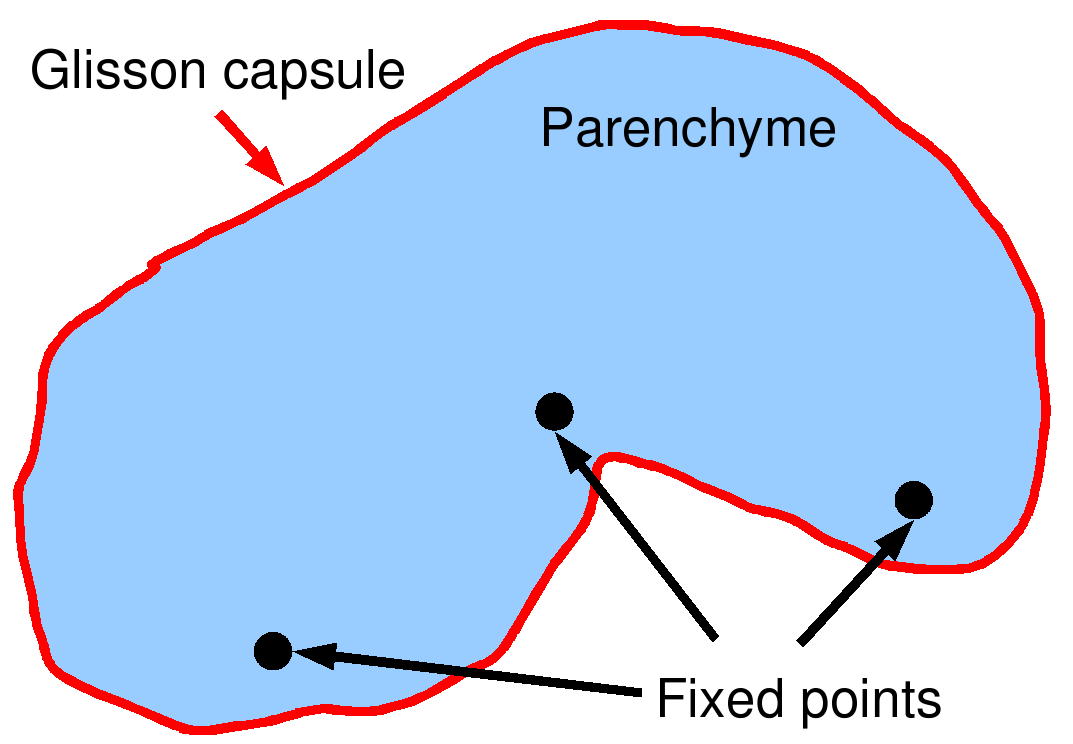
\includegraphics[width=\linewidth]{liver_2ForceFields.png}
\item inside: soft material
\item surface: stiffer material
\end{itemize}

\column[t]{0.5\linewidth}
A specialized program:
\lstset{basicstyle=\large}
\begin{code_cpp}
f = M*g
f += F1(x,v)
f += F2(x,v)
a = f/M
a = C(a)
v += a * dt
x += v * dt
display(x)
\end{code_cpp}

\end{columns}

\end{frame}



%-----------------------------------------
\begin{frame}
\frametitle{Component-based simulation object }
\begin{columns}
 \column[c]{0.5\linewidth}
%Data:
\begin{itemize}
\item<1-> state vectors (DOF): $x,v,a,f$
\item<1-> constraints: fixed points 
\only<1> {\\ \em other: oscillator, collision plane, etc.}
\item<2-> force field: tetrahedron FEM
\only<2> {\\ \em other: triangle FEM, springs, Lennard-Jones, SPH, etc.}
\item<3-> force field: triangle FEM
\item<4-> mass: uniform
\only<4> {\\ \em other: diagonal, sparse symmetric matrix}
\item<5-> ODE solver: explicit Euler
\only<5> {\\ \em other: Runge-Kutta, implicite Euler, static solution, etc.}
\end{itemize}
 \column[c]{0.5\linewidth}
\only<1>{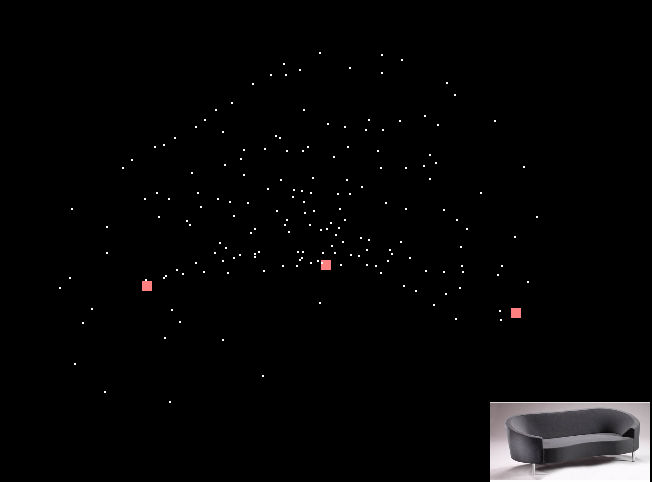
\includegraphics[width=0.9\linewidth]{liverDOF.png}\\ 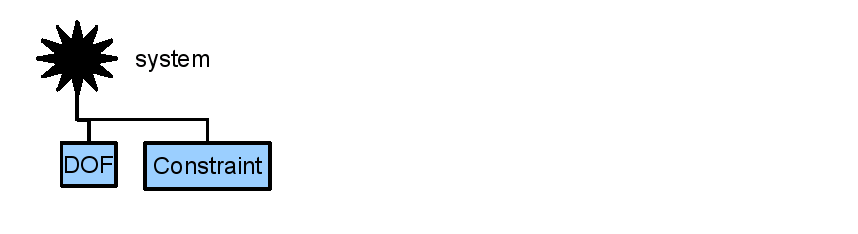
\includegraphics[width=\linewidth]{layeredLiver3-tree-1.png}}
\only<2>{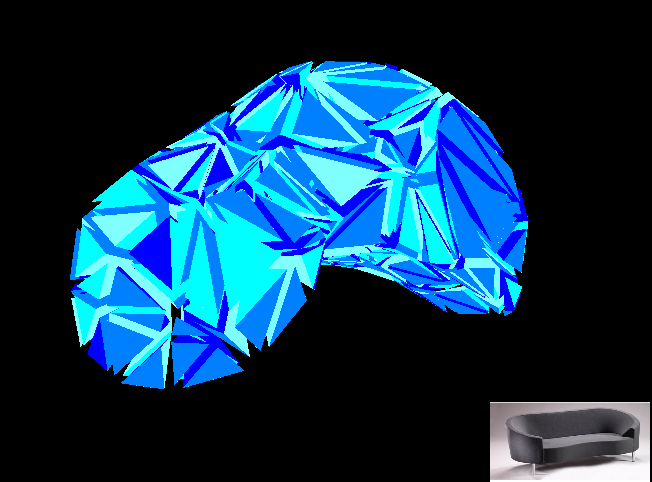
\includegraphics[width=0.9\linewidth]{liverTetra.png}\\ 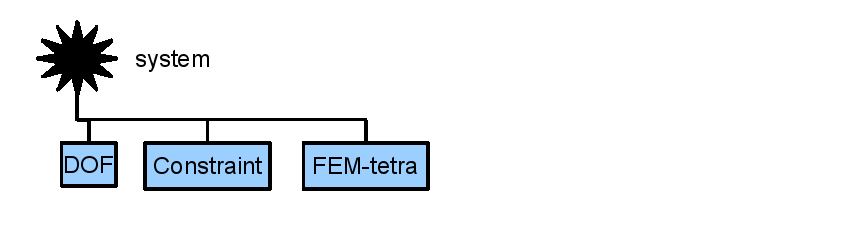
\includegraphics[width=\linewidth]{layeredLiver3-tree-2.png}}
\only<3>{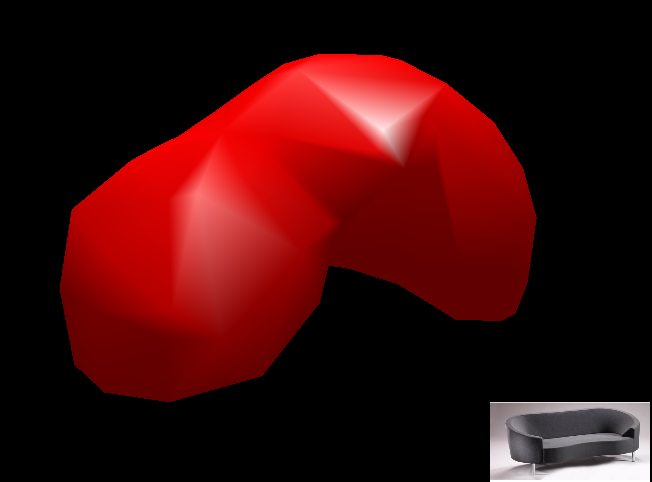
\includegraphics[width=0.9\linewidth]{liverTrian.png}\\ 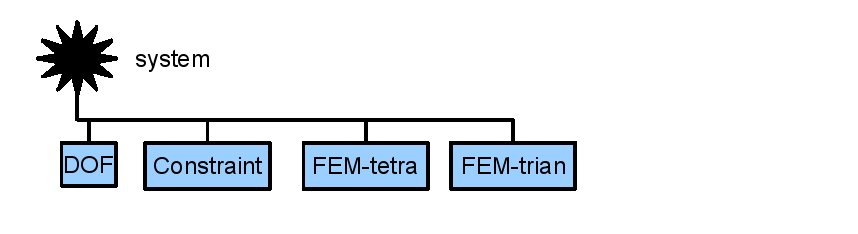
\includegraphics[width=\linewidth]{layeredLiver3-tree-3.png}}
\only<4>{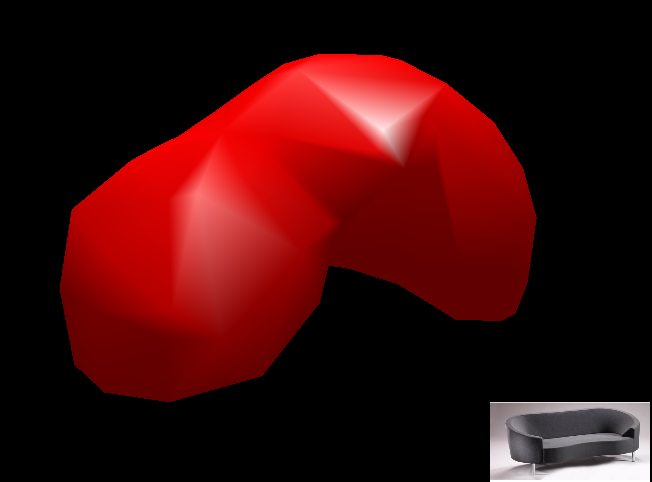
\includegraphics[width=0.9\linewidth]{liverTrian.png}\\ 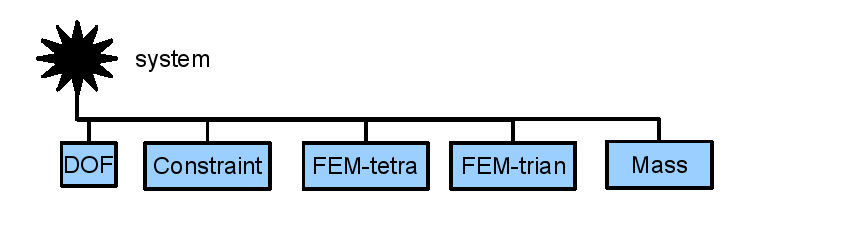
\includegraphics[width=\linewidth]{layeredLiver3-tree-4.png}}
\only<5>{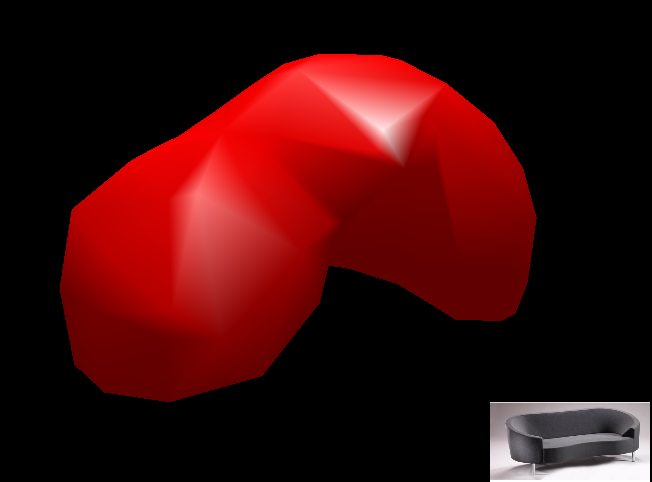
\includegraphics[width=0.9\linewidth]{liverTrian.png}\\ 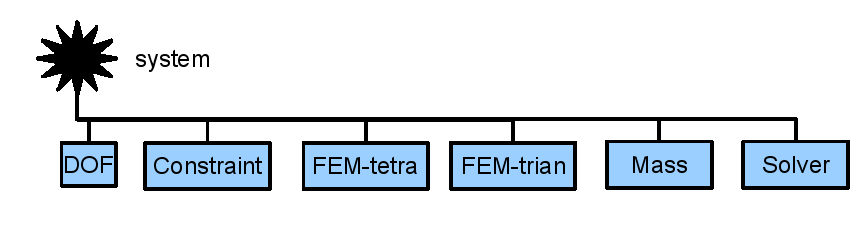
\includegraphics[width=\linewidth]{layeredLiver3-tree-5.png}}
\end{columns}
\end{frame}

%-----------------------------------------
\begin{frame}
\frametitle{Actual decomposition}
\includegraphics[width=0.9\linewidth]{snapshot1.png}

\end{frame}

%-----------------------------------------
\begin{frame}
\frametitle{Multiphysics}
Non-mechanical solvers can be coupled with the simulation


\includegraphics[width=0.99\linewidth]{mechanical-electrical.png}

\end{frame}

%-----------------------------------------
\begin{frame}
\frametitle{Operations}

\begin{itemize}
 \item The ODE solver sends visitors to apply operations
 \item The visitors traverse the scene and apply virtual methods to the components
 \item The methods read and write state vectors (identified by symbolic constants) in the DOF component
 %\item State vectors are identified by symbolic constants 
 \item Example: accumulate force
  \begin{itemize}
   \item A \texttt{ResetForceVisitor} recursively traverses the nodes of the scene (only one node here)
  \begin{itemize}
   \item All the \texttt{DOF} objects apply their \texttt{resetForce()} method
  \end{itemize}
   \item An \texttt{AccumulateForceVisitor} recursively traverses the nodes of the scene 
  \begin{itemize}
   \item All the \texttt{ForceField} objects apply their \texttt{addForce(  Forces, const Positions, const Velocities )} method
  \end{itemize}
   \item the final value of f is weight + tetra fem force + trian fem force
  \end{itemize}
\end{itemize}

\end{frame}

% %-----------------------------------------------
% \begin{frame}[fragile]
% \frametitle{Object-oriented hierarchical structure}
% \begin{columns}
% \column[c]{0.5\linewidth}
% \begin{itemize}
%  \item The system aggregates abstract components
%  \item The components are independent
% \item
%  \only<2>{\item Force fields: springs, triangle FEM, tetrahedron FEM, SPH, etc.}
%  \only<3>{ Constraints: fixed points, oscillators, half-space, etc.}
%  \only<4>{\item Mass: uniform, diagonal, symmetric sparse matrix}
%  \only<5>{\item Solver: explicit Euler, implicit Euler, Runge-Kutta, static, etc. }
% 
%  \item They communicate through the system
%  \item The solver triggers \textit{actions}
% \end{itemize}
% 
%  \column[c]{0.5\linewidth}
% \includegraphics[width=\linewidth]{system_simple.png}
% \end{columns}
% \end{frame}



%%%===================================================================
\section{Software development}
%%%===================================================================

\begin{frame}
 \frametitle{Implementation}
\begin{itemize}
 \item C++ libraries 
 \item Linux, Windows, Mac
 \item 800,000 lines of code
 \item 138,000 downloads
\end{itemize}

\end{frame}



\begin{frame}
 \frametitle{Contributors}
 80 contributors to the code. Three full-time engineers.
\begin{itemize}
 \item Cimit (Boston)/Graphix (Lille)
 \item Evasion/Imagine (Grenoble)
 \item Epidaure/Asclepios (Sophia-Antipolis)
 \item Shacra (Strasbourg)
 \item MOAIS (Grenoble), Sed Sophia, …
 \item Companies: Digital Trainers, Bellcurves, InSimo, …
\end{itemize}

\end{frame}

\begin{frame}
 \frametitle{Features}
\begin{itemize}
 \item deformable solids: FEM, cables, frame-based,…
 \item mass-springs, rigid, SPH
 \item soft, stiff, hard constraints
 \item iterative and direct solvers
 \item collision detection and response
 \item multiphysics
\end{itemize}

\end{frame}




%%%===================================================================
\section{Conclusion}
%%%===================================================================


\begin{frame}
 \frametitle{Conclusion - Features}
High modularity:
\begin{itemize}
 \item Abstract components: DOF, Force, Constraint, Solver, Topology, Mass, CollisionModel, VisualModel, etc. 
 \item Multimodel simulations using mappings
 \item Explicit and implicit solvers, Lagrange multipliers
\end{itemize}
Efficiency:
\begin{itemize}
 \item global vectors and matrices are avoided
 \item parallel implementations
\end{itemize}
Implementation:
\begin{itemize}
 \item currently $450,000$ C++ lines
 \item Linux, MacOs, Windows
\end{itemize}

\end{frame}


%-----------------------------------------------

\begin{frame}
\frametitle{Ongoing work}
\begin{itemize}
\item models and algorithms: better numerical solvers, cutting, haptics, Eulerian fluids...
\item asynchronous simulation/rendering/haptic feedback 
\item multiphysics (electrical/mechanical)
\item parallelism for everyone
\item more documentation
\end{itemize}
% \end{frame}
% 
% \begin{frame}
% \frametitle{Applications}

\vspace{1cm}
\begin{center}
\Large
 www.sofa-framework.org
\end{center}


\end{frame}




\end{document}


